%Matteo Kumar - Leonard Schatt
% Fortgeschrittenes Physikalisches Praktikum

\clearpage
\section{Fitten der Shockley-Gleichung}
\label{chapter:fitten}

Aus den Daten wurde mithilfe einens MatLab-Programmes ref die Parameter, welche in der Shockley-Gleichung vorkommen ref gefittet. Dabei wird beachtet, 
dass bei der CIS-Zelle einen Reihenschaltung von 11 kleinen Solarmodulen vorhanden ist. Daher wird die Spannung durch 11 geteilt. Leider erhält man 
trotzdem sehr fragwürdige Parameter, beispielsweise unrealistisch hohe Temperaturen als Umgebungsbedingungen hatten. Diese sind aber ausgeschlossen, 
da die Temperatur als Referenz gemessen wurde.
Interessant ist vor allem, dass sich mit dem Programm vor allem die Multi- und MonoSi besser mit der Shockley-Gleichung gefittet werden, als 
die CIS Solarzelle, was aber auch gut an der fehlerhaften Anwendung des Programmes oder dem Programm selbst.

\subsection{CIS-Solarmodul}

Nach dem Fitten mit dem oben erwähnten Programm erhält man folgende Abbildungen und Parameter.

\begin{figure}[ht]
    \centering
    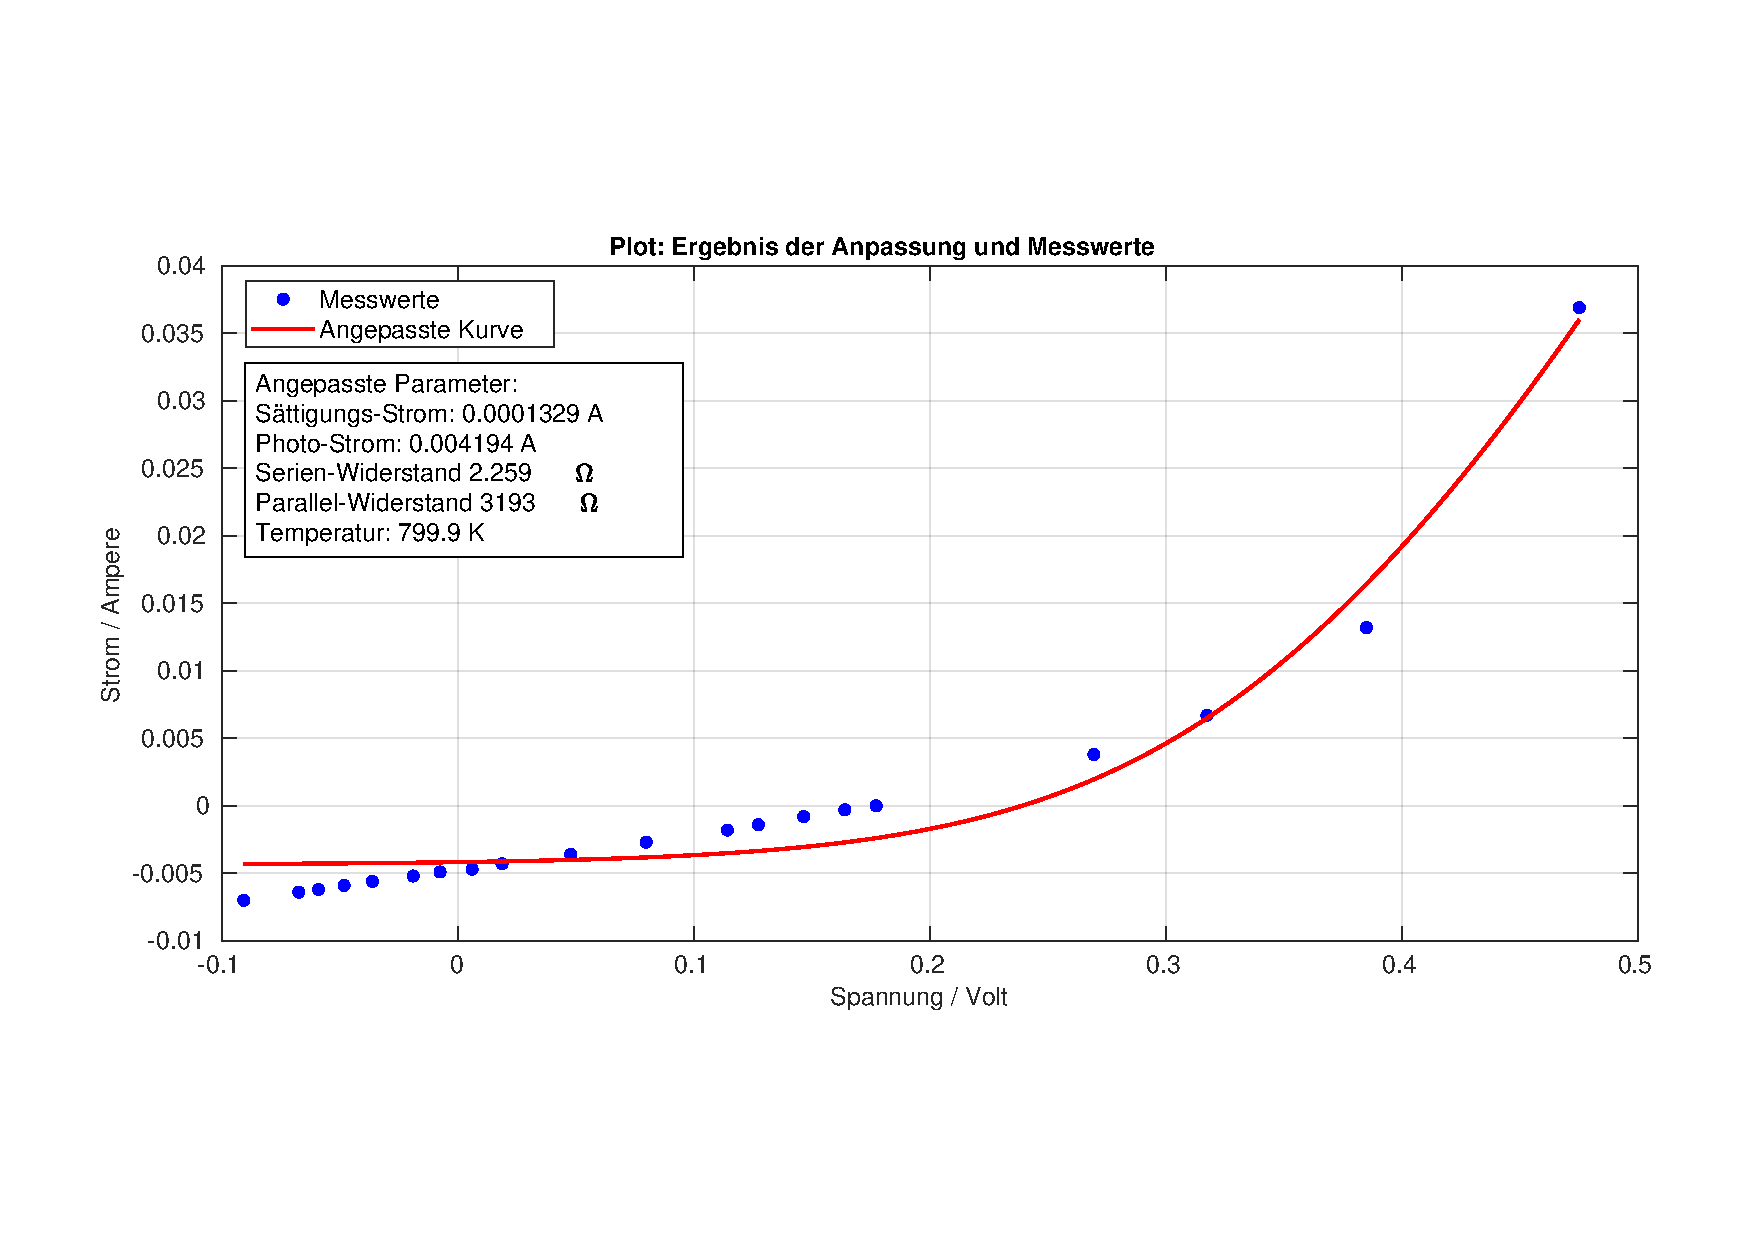
\includegraphics[width = \linewidth]{Bilder/CIS130Plot.pdf}
    \caption{Gefittete Shockley-Gleichung an das CIS-Modul bei 130V Trafospannung}
    
\end{figure}


Dabei fällt vor allem die ungewöhnlich hohe Temperatur. Der Reihenwiderstand ist größer als der der anderen Module. Dies ist jedoch normal, da 
es ja auch 11 Module sind und somit 11 Mal die entsprechenden Kontaktstellen existieren. Der Parallelwiderstand ist groß, was aber ein gutes 
Zeichen ist, weil das bedeutet, dass der Leckstrom gering ist.\\
Im Gesamten muss man sagen, dass sich bei dem CIS-Modul kein schöner exponentieller Zusammenhang finden lässt. Nicht desto trotz ist dieser 
eine ausreichend gute Beschreibung der Wirklichkeit um Aussagen über die CIS-Zelle zu machen.

Bei allen Solarzellen finden sich die Fits im Anhang \ref{section:AnhangShock}.




\subsection{Mono- und MultiSi-Zellen}

Auch Mono- und MultiSi-Module wurden versucht mit dem Programm zu fitten. Dabei funktionierte das hier sichtlich besser.

\begin{figure}[ht]
    \centering
    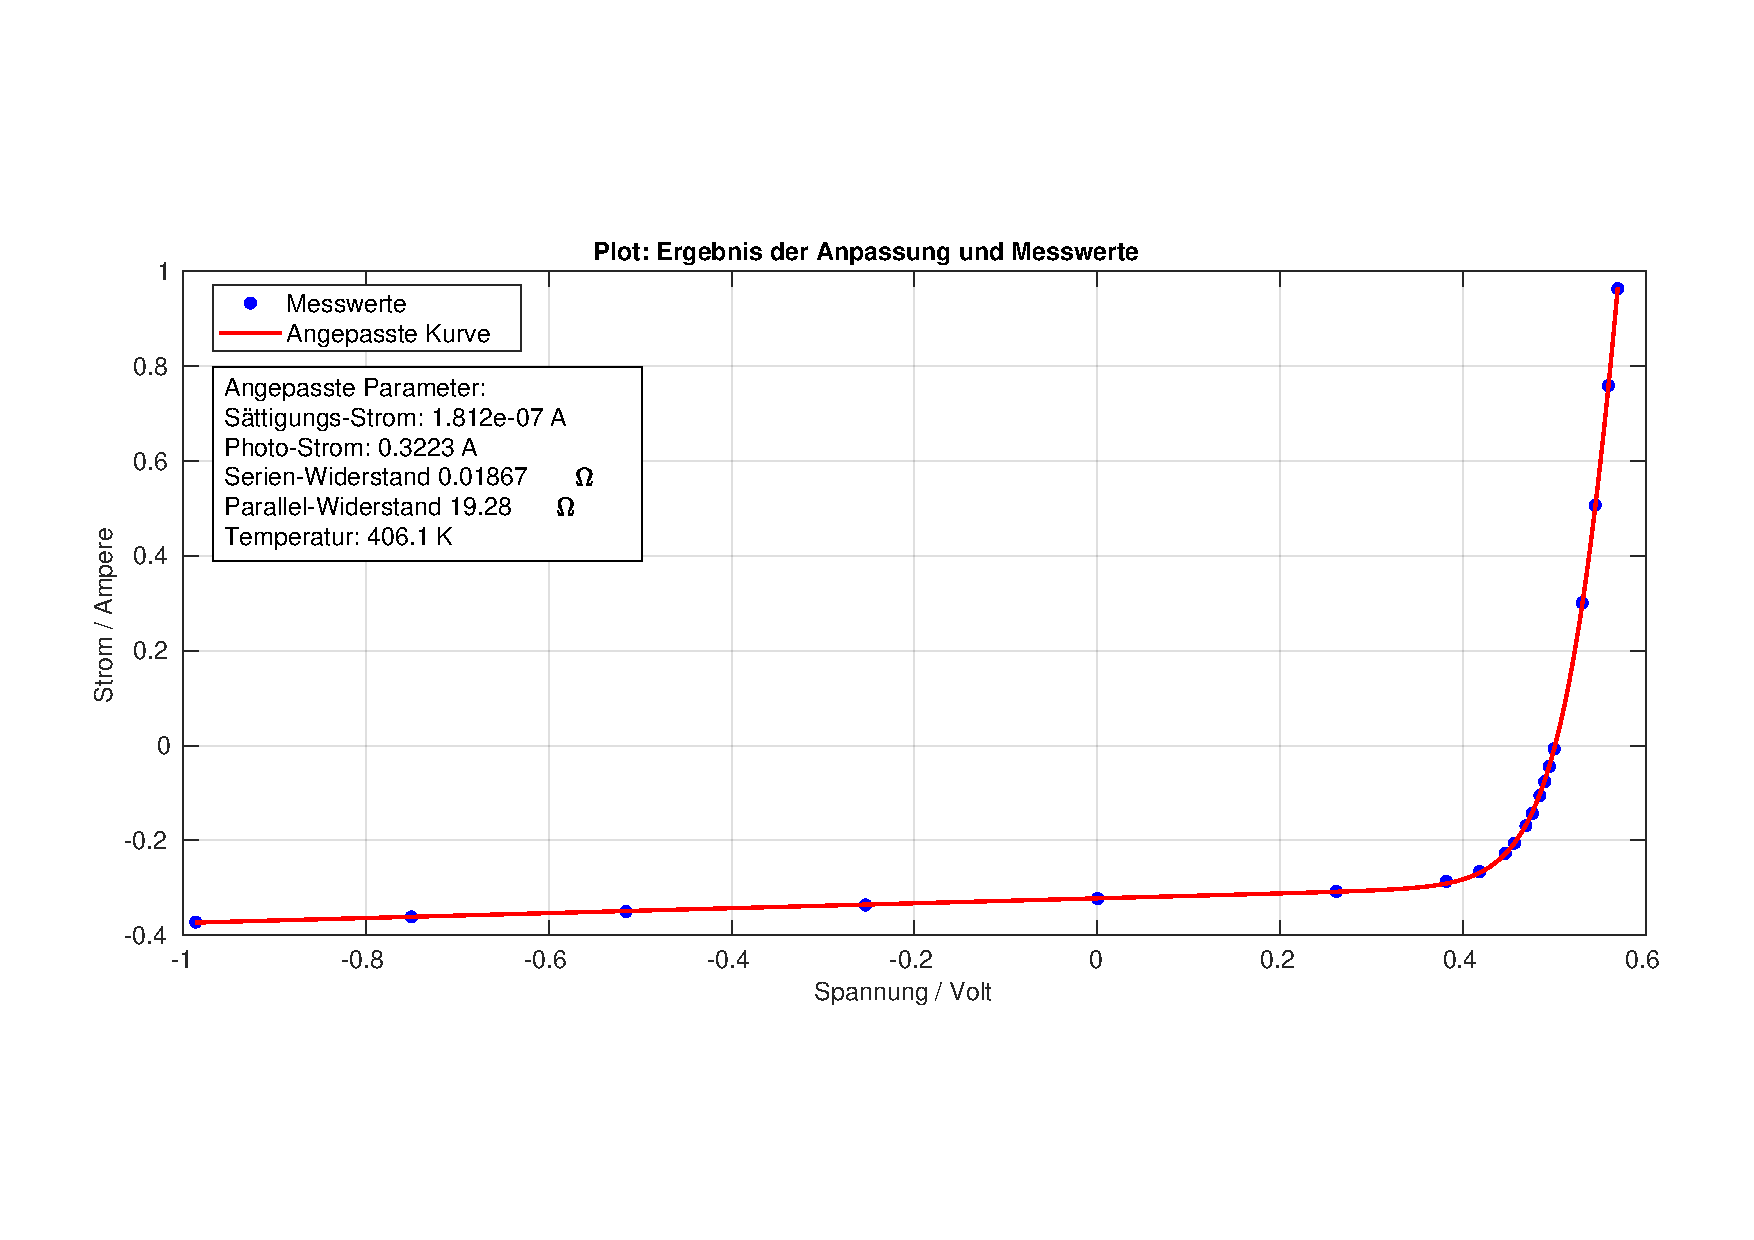
\includegraphics[width = \linewidth]{Bilder/SiMono130Plot.pdf}
    \caption{Gefittete Schockley-Gleichung an das Mono-Si-Modul bei 130V}
\end{figure}

\begin{figure}[ht]
    \centering
    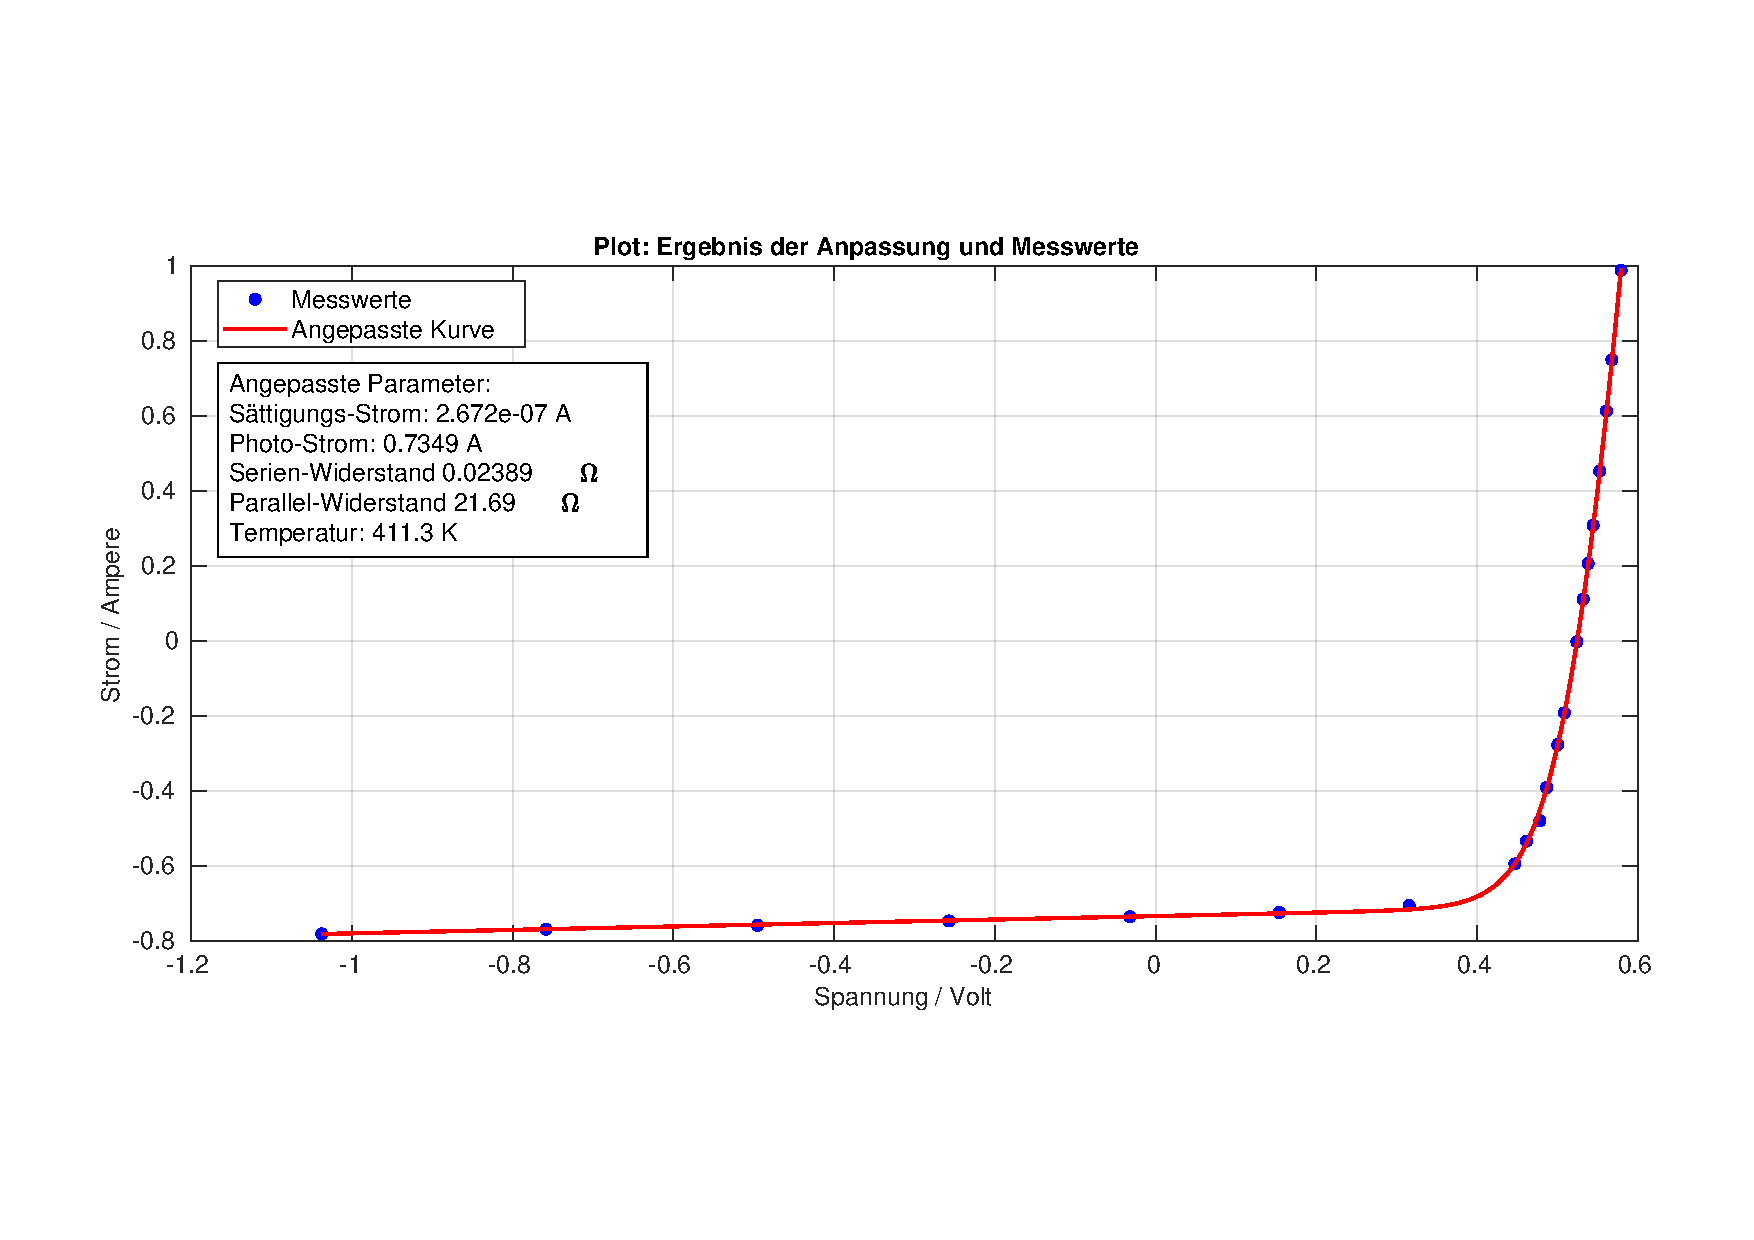
\includegraphics[width = \linewidth]{Bilder/SiMono180Plot.pdf}
    \caption{Gefittete Schockley-Gleichung an das Mono-Si-Modul bei 180V}
\end{figure}


\begin{figure}[ht]
    \centering
    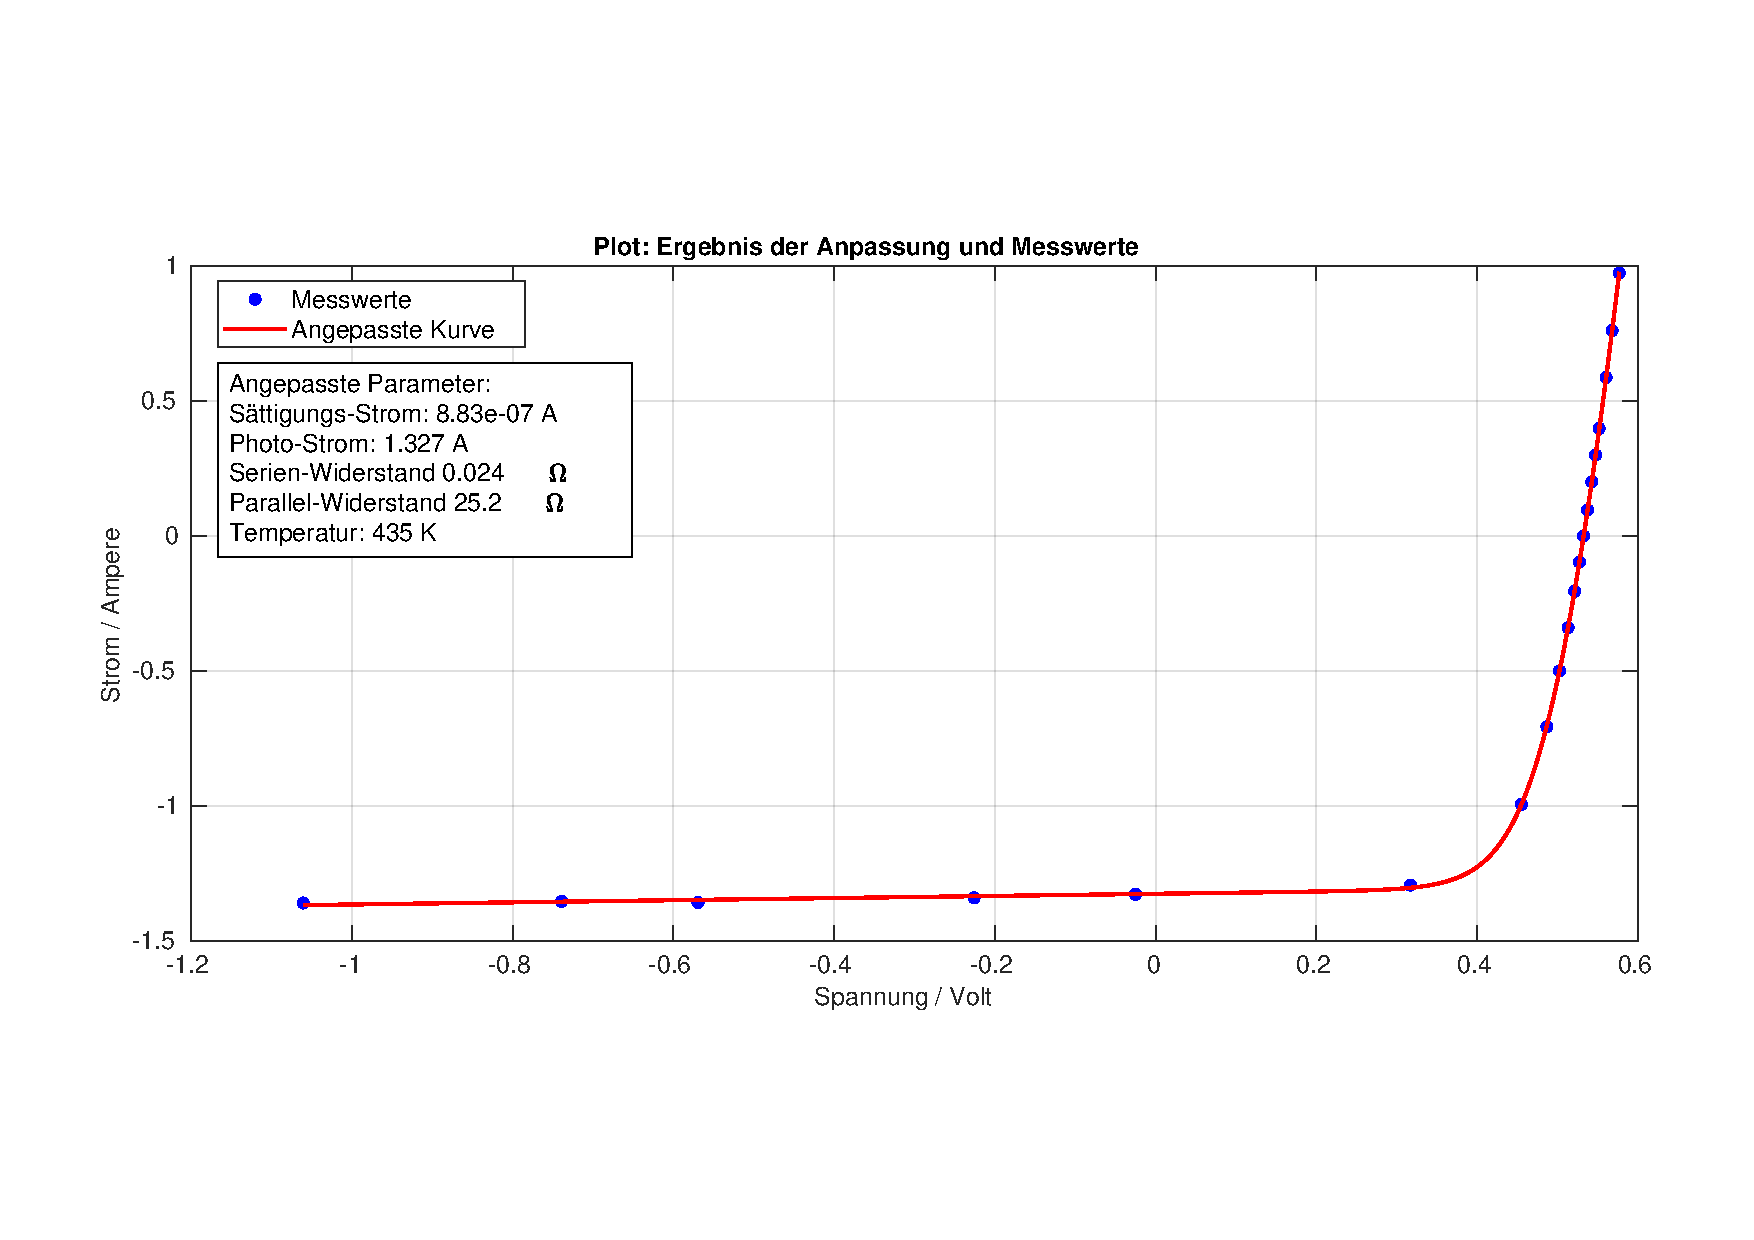
\includegraphics[width = \linewidth]{Bilder/SiMono230Plot.pdf}
    \caption{Gefittete Schockley-Gleichung an das Mono-Si-Modul bei 230V}
\end{figure}


Dabei ist, wie erwartet, der Photostrom $I_{Ph}$ bei steigender Helligkeit immer stärker. Die restlich Grafiken befinden sich im Anhang. Bei 
allen ist schön das "nach unten verschieben" bei höherer Lichtleistung beobachtbar. \\
Die Füllfaktoren $FF$ und Strom und Spannung am $MPP$ ergeben sich nach grafischer Auswertung. Dabei wird mit dem Computer das U-I-Paar gesucht, welches die maximale Fläche 
im vierten Quadranten der U-I-Ebene einschließt. Um den Füllfaktor zu erhalten werden dann noch $U_{OC}$ und $I_{Ph}$ bestimmt und dann wird dieser wie in den Grundlange 
beschrieben errechnet. Damit erhält man folgende Werte :\\
\begin{table}[h]
    \centering
    \begin{tabular}{l|c|c|r}
        & Spannung am $MPP$ (V) & Strom am $MPP$ (A) & $FF$ \\
        \toprule
        SiMono bei 130V & 0.405 & -0.27 & 0.69 \\
        SiMono bei 180V & 0.416 &-0.66 & 0.71 \\
        SiMono bei 230V & 0.412 & -1.19 & 0.69\\
        \midrule
        SiMulti bei 130V & 0.398 & -0.25 & 0.70 \\
        SiMulti bei 180V & 0.414 & -0.55 & 0.71 \\
        SiMulti bei 230V & 0.435 & -1.05 & 0.74\\
        \midrule
        CIS bei 130V & 0.151 &  -0.0029 & 0.44 \\
        CIS bei 180V & 0.202 & -0.0073 & 0.48 \\
        CIS bei 230V & 0.238 & -0.0144 & 0.51\\
    \end{tabular}
\end{table}

Dabei ist auffällig, dass am $MPP$ die Spannungswerte immer nahezu identisch sind. Die Stromwerte steigen aber eindeutig. Außerdem ist der 
niedrige Füllfaktor bei den CIS-Modul auffällig. Daraus würde man ein langsames Ansteigen der Kurve vermuten, welches man dann im Bild auch beobachten kann. 
Die CIS-Zelle ist somit am weitesten von einer idealen Solarzelle entfernt, da sie den langsamen Anstieg hat. Das erklärt auch, warum beim fitten die 
hohe Temperatur vorgeschlagen wird, da diese zu einem langsameren Anstieg der U-I-Kennlinie führt. Insgesamt beschreibt das Ersatzschaltbild 
die CIS-Zelle möglicherweise nicht gut.

\clearpage

\subsection{Idealitätsfaktor}

Der Idealitätsfaktor $n$ ist ein Faktor, der beschreibt, wie gut sich der Halbleiter, beziehungsweise hier der pn-Übergang durch das Bändermodell 
darstellen lässt. Dabei kann man diesen relativ einfach aus der Shockley-Gleichung gewinnen.

\begin{equation}
    n =  \frac{qU}{kT} \frac{1}{\ln{(\frac{I_{Ph}+\frac{R_S I -U}{R_P}+I}{I_0}+1)}}
    \label{Ideal1}
\end{equation}

Bei der Gleichung ist $I_0$ der Sättigungsstrom, $I_{PH}$ der Fotostrom, $U$ die Spannung, $R_{S}$ und $R_{P}$ der Reihen- und Parallelwiderstand.\\
Gleichung \ref{Ideal1} kann man nochmal vereinfachen, indem man an der Stelle (U,I)= ($U_{OC}$,0A) einsetzt.

\begin{equation}
    n =  \frac{qU}{kT} \frac{1}{\ln{(\frac{I_{Ph}-\frac{U_{OC}}{R_P}}{I_0}+1)}}
    \label{Ideal2}
\end{equation}

Setzt man die in Kapitel \ref{chapter:fitten} erhaltenen Werte ein, so erhalt man als Idealitätsfaktoren die folgenden Werte.

\begin{table}[h]
    \centering
    \begin{tabular}{l|r}
        MonoSi-Modul & $n$ = 1.004\\
        MultiSi-Modul & $n$ = 1.004\\
        CIS-Modul & $n$ = 1.003\\
    \end{tabular}
    \caption{Idealitätsfaktoren der Solar-Module }
\end{table}

Wie bei den obigen Werten ist es schwer überhaupt Fehler anzugeben, da die einzelnen Parameter aus der Shockley-Gleichung 
schwer im Fehler abzuschätzen sind. Eine Unsicherheit von 10\% wäre jedoch sicher nicht untertrieben.\
Im Gesamten kann man sagen, dass die obigen Werte durchaus realistisch erscheinen. Eine 
Diode sollte einen Idealitätsfaktor zwischen 1-2 haben. Hier liegen wir schon nah an 1, dass 
heißt, dass sich die Solar-Module sehr gut durch das Bändermodell beschreiben lassen.


\subsection{Wirkungsgrad}

Eine spannende Frage ist nun, wie es sich mit dem Wirkungsgrad in Abhängigkeit von der Beleuchtungsstärke verhält. 
Dabei berechnet man die Lichtintensität aus den Referenzmessungen mit der kalibrierten Solarzelle. Mithilfe dieser 
bestimmt man die Lichtleitung $P_L$. Der Wirkungsgrad $\eta$ ergibt sich dann wie im theoretischen Teil beschrieben. 

\begin{figure}[h]
    \centering
    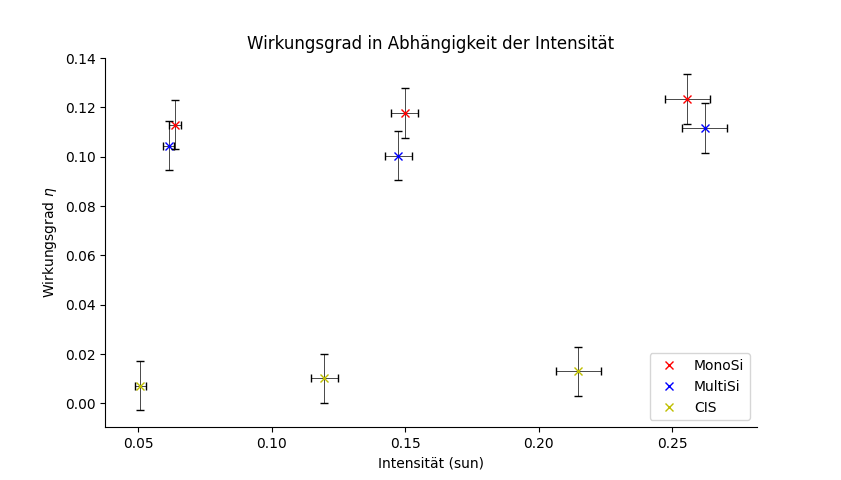
\includegraphics[width = \linewidth]{Bilder/WirkungsgradInt.png}
    \caption{Wirkungsgrad verschiedner Solarmodule bei Intensitäten bis zu 0,25\,sun. Die Fehler sind Fehlerabschätzungen, 
    beispielsweise für die X-Werte aus der Schwankung der Intensität bei der Messung mir der geeichten Solarzelle}
\end{figure}

Dabei kann man einen Trend zu einem besseren Wirkungsgrad bei höheren Frequenzen sehen. Dies ist vermutlich ein 
temperaturbedingter Effekt, da die Module bei höheren Intensitäten deutlich wärmer wurden. Des Weiten sieht man schön den Unterschied 
im Wirkungsgrad zwischen der MonoSi- und der MultiSi-Solarzelle. Die monokristalline Solarzelle hat, wie erwartet, einen etwas höheren 
Wirkungsgrad. Dabei sind beide etwas zu hoch angesiedelt. 
Die CIS-Zelle hingegen hat einen deutlich zu niedrigen Wirkungsgrad, was realistisch schein, da diese immer ein bisschen schlechter als die beiden obigen Module 
sein sollte. Es ist realistisch, dass man bei Werten unter 20\% bleibt für den Wirkungsgrad.\

Auffällig ist dabei noch, dass die Spannung $U_{OC}$ relativ konstant bleibt, der Photostrom hingegen linear mit der Beleuchtungsstärke zunimmt. 
Im Gesamten bleibt die Form der Kurve jedoch ähnlich, was man auch an konstanten Füllfaktoren sieht. Die Grafiken dazu im Anhang.


\subsection{Extrapolieren der Photostroms}

Der Photostrom $I_{Ph}$ wird bis 1sun extrapoliert. Dabei wird ein linearer Zusammenhang angenommen, da eine Zunahme der Lichtintensität direkt proportional zu der 
Anzahl der Photonen ist. Der Photostrom hängt von der Anzahl der Elektronen ab, die durch den photoelektrischen Effekt zum Photostrom beitragen können. Diese ist proportional zur 
Anzahl der eintreffenden Photonen. Durch lineare Regression ergibt sich das folgende Bild für die extrapolierten Werte.
\begin{figure}[h]
    \centering
    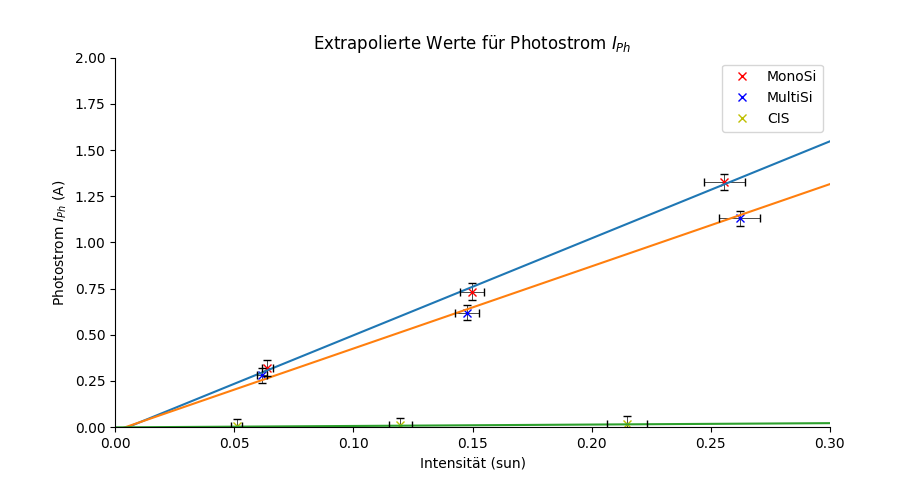
\includegraphics[width = 12cm]{Bilder/ExtraInt.png}
    \caption{Ausschnitt der obigen Abbildung}
\end{figure} 

Dabei sieht man, dass die Daten sehr gut in einen linearen Zusammenhang zu setzen sind. Die extrapolierten Werte für 1 sun sind in Tabelle \ref{tabelle:Interpol}.
\begin{table}[ht]
    \centering
    \begin{tabular}{lr}
        Solarzellenart & Extrapolierter Wert\\
        \midrule
        CIS & 0,07\,A\\
        MonoSi&5,2\,A\\
        MultiSi&4,4\,A\\
    \end{tabular}
    \caption{Interpolierte Werte der drei Solarzellen bei 1\,sun}
    \label{tabelle:Interpol}
\end{table}
